\documentclass[11pt]{article}

\title{4C8 Lab 1 - Pixel Operations}
\author{Jonathan Kearney (14313977)}


\usepackage{graphicx}
\usepackage{geometry}
\usepackage{verbatim}
\usepackage{multicol}
\usepackage[hidelinks]{hyperref}
\usepackage{float}
\usepackage{physics}
\usepackage{verbatim}
\usepackage[parfill]{parskip}
\usepackage{cite}
\usepackage{amsmath}
\usepackage{multirow}
\usepackage{pdfpages}
\usepackage{tikz}
\usepackage{xcolor}
\usepackage{siunitx}
\usepackage{caption}
\usepackage{subcaption}
\usepackage{forest}
\usepackage{pgfgantt}
\usepackage{rotating}
\usepackage{tabu}
\usepackage{lmodern,textcomp}
\usepackage{eurosym}
\usepackage{siunitx}


\geometry{margin = .85in}





\begin{document}

%TITLE PAGE
\maketitle



%ABSTRACT	



\newpage


%IMAGE LOADING AND DISPLAY
\section{Basic Image Loading and Display}
Lennna.256 was loaded into Matlab. This displayed a greyscale image as seen in Figure \ref{Lenna} (a). Each value in the matrix represented a pixel and contained a number between 0 and 255 (0 = black and 255 = white). When 128 was added onto each element in the matrix, every pixel was closer to 255. Therefore, this made the image appear brighter than the original, as in Figure\ref{Lenna} (b). When 128 was subtracted from every pixel in the matrix, then each element had a value closer to 0 and the image appeared darker than the original.

\begin{figure}[H]
\centering
\begin{subfigure}{.49\textwidth}
	\centering
        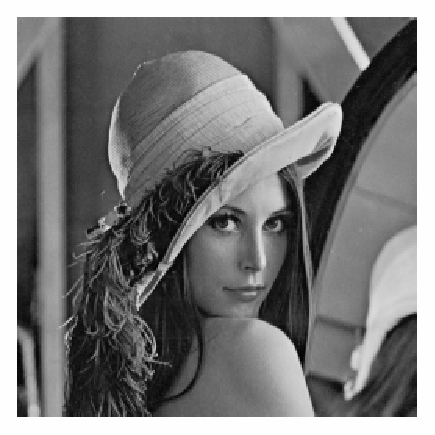
\includegraphics[width=\linewidth, height = 7cm]{pic.eps}
        \caption{}
        \label{normal}
\end{subfigure}
\begin{subfigure}{.49\textwidth}
	\centering
        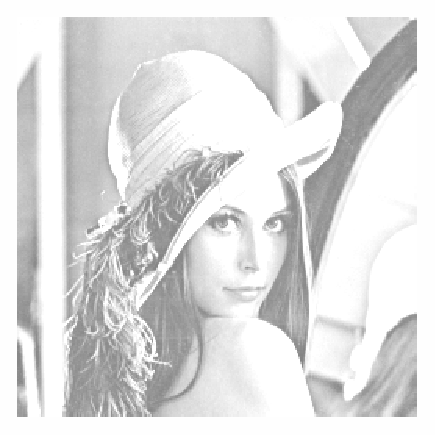
\includegraphics[width=\linewidth,  height = 7cm]{newpic1.eps}
        \caption{}
        \label{brighter}
\end{subfigure}
\begin{subfigure}{.49\textwidth}
	\centering
        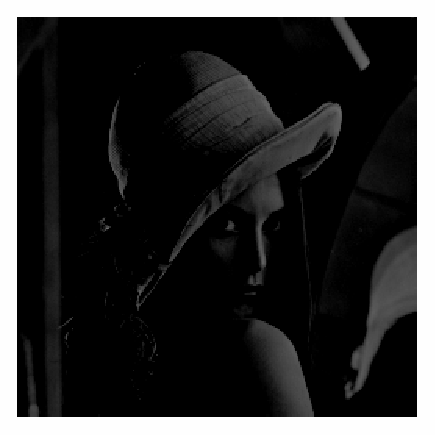
\includegraphics[width=\linewidth, height = 7cm]{newpic2.eps}
        \caption{}
        \label{darker}
\end{subfigure}
\caption{(a): Normal unedited picture, (b): Picture with 128 added onto matrix, therefore displaying brighter, (c): Picture with 128 subtracted from image, hence displaying a darker image.}
\label{Lenna}
\end{figure}



% HISTOGRAMS

\section{Histograms}

\subsection{Image Size}
The image sigmedia06907.tif was loaded into Matlab. This image was read in as a colour image of size 576x720x3. However, this was converted to greyscale in Matlab, hence removing the 3 colour planes. Once this was completed, the size of the resulting picture was checked using the size() function. This returned a value of 576x720. This meant that the picture was 576 pixels tall (576 matrix rows) and 720 pixels wide (720 matrix columns). As the image is in greyscale, the third dimension of three is removed.

\subsection{Pool Table Histograms}
Figure \ref{pool} shows the 3 histograms (Red, Green and Blue) for the image `pool.01.bmp'. In Figure \ref{pool} (a) the histogram for the red plane can be seen. There is a clear spike in the graph in the range 50-100. There are similar spikes in plot (b) (Green) from 120-180 and (c) (Blue) from 30-70. These spikes correspond to the tabletop of the pool table in the image. As the table makes up a large proportion of the image, the highest values of Red, Green and Blue in the histograms will be dedicated to this region. Therefore the table is portrayed by the spikes in the graphs. 

\begin{figure}[H]
\centering
\begin{subfigure}{.49\textwidth}
	\centering
        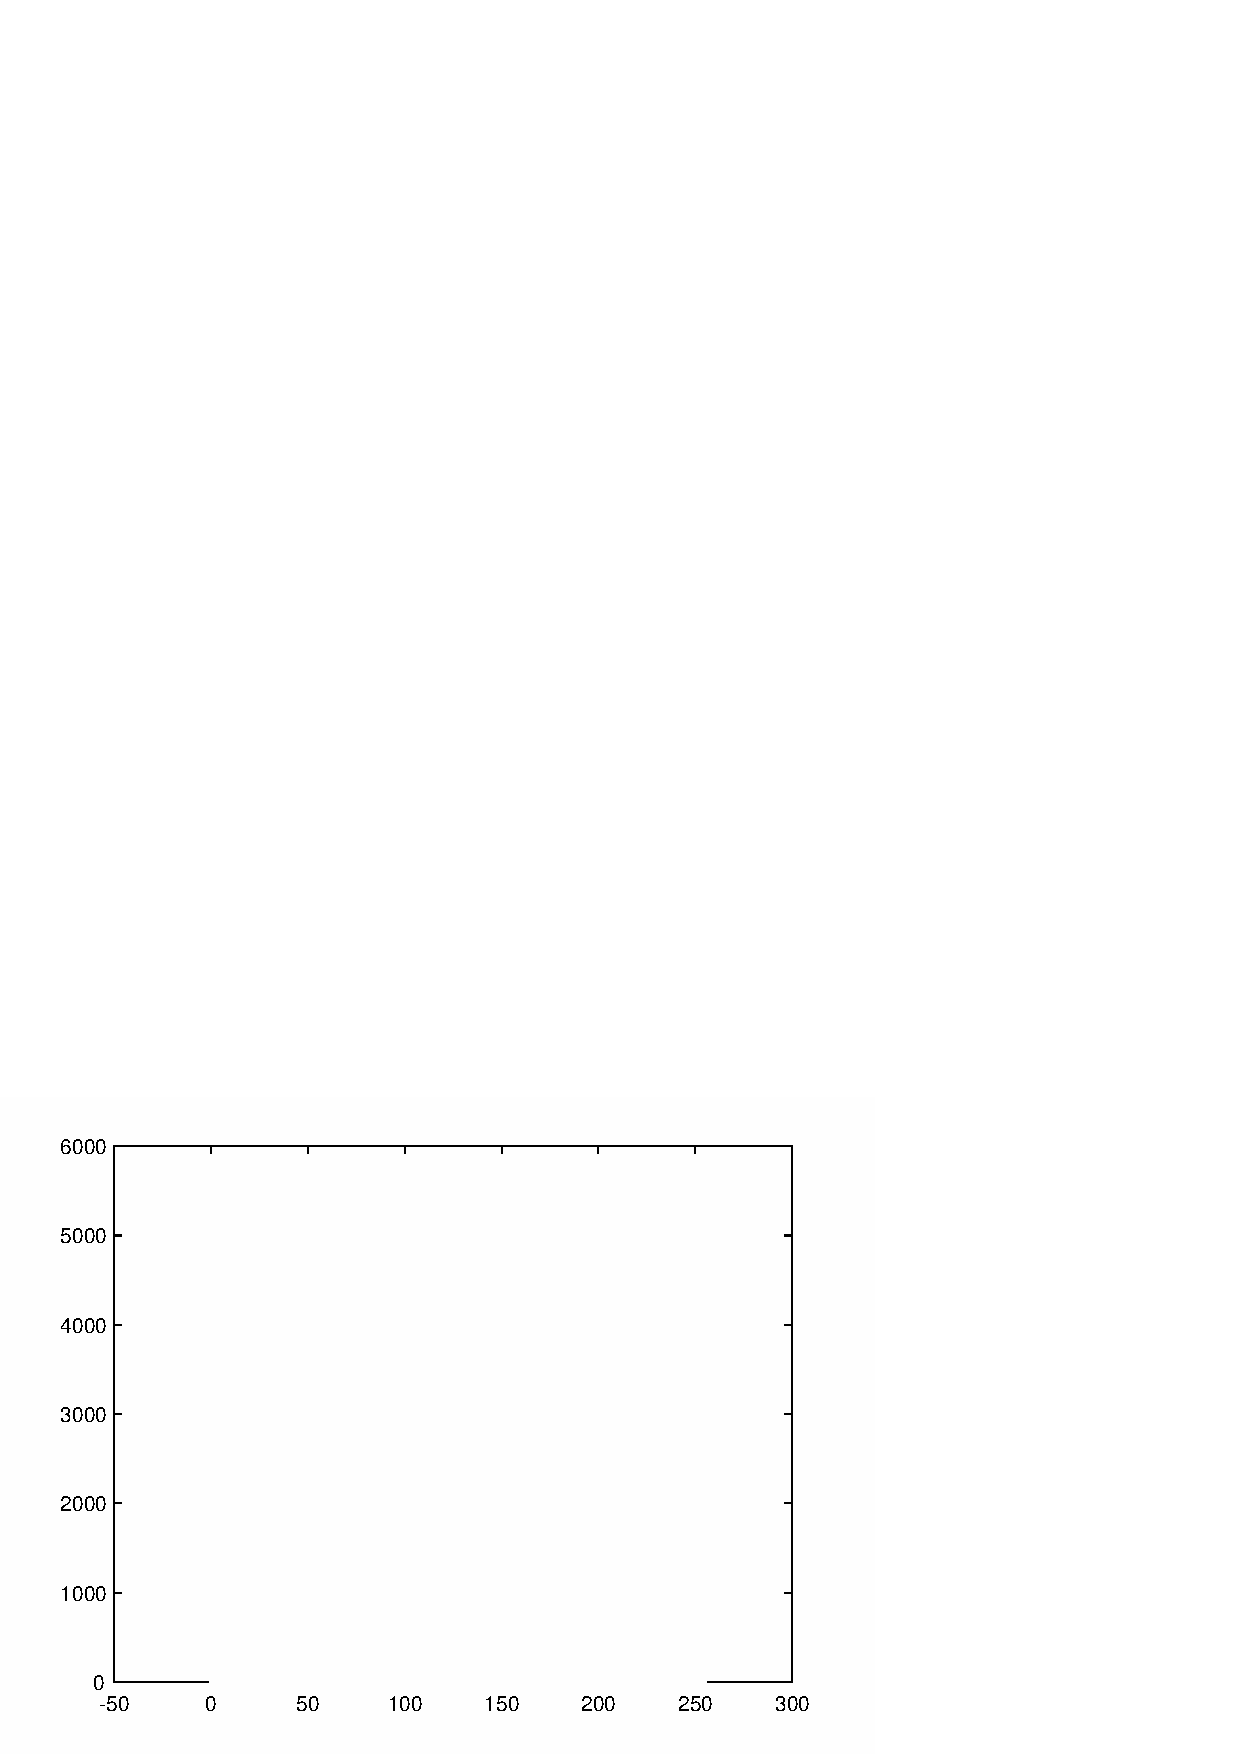
\includegraphics[width=\linewidth, height = 5.5cm]{redplane.jpg} %.eps didn't show the colour of the histogram graphs so .jpg is used instead
        \caption{}
        \label{red}
\end{subfigure}
\begin{subfigure}{.49\textwidth}
	\centering
        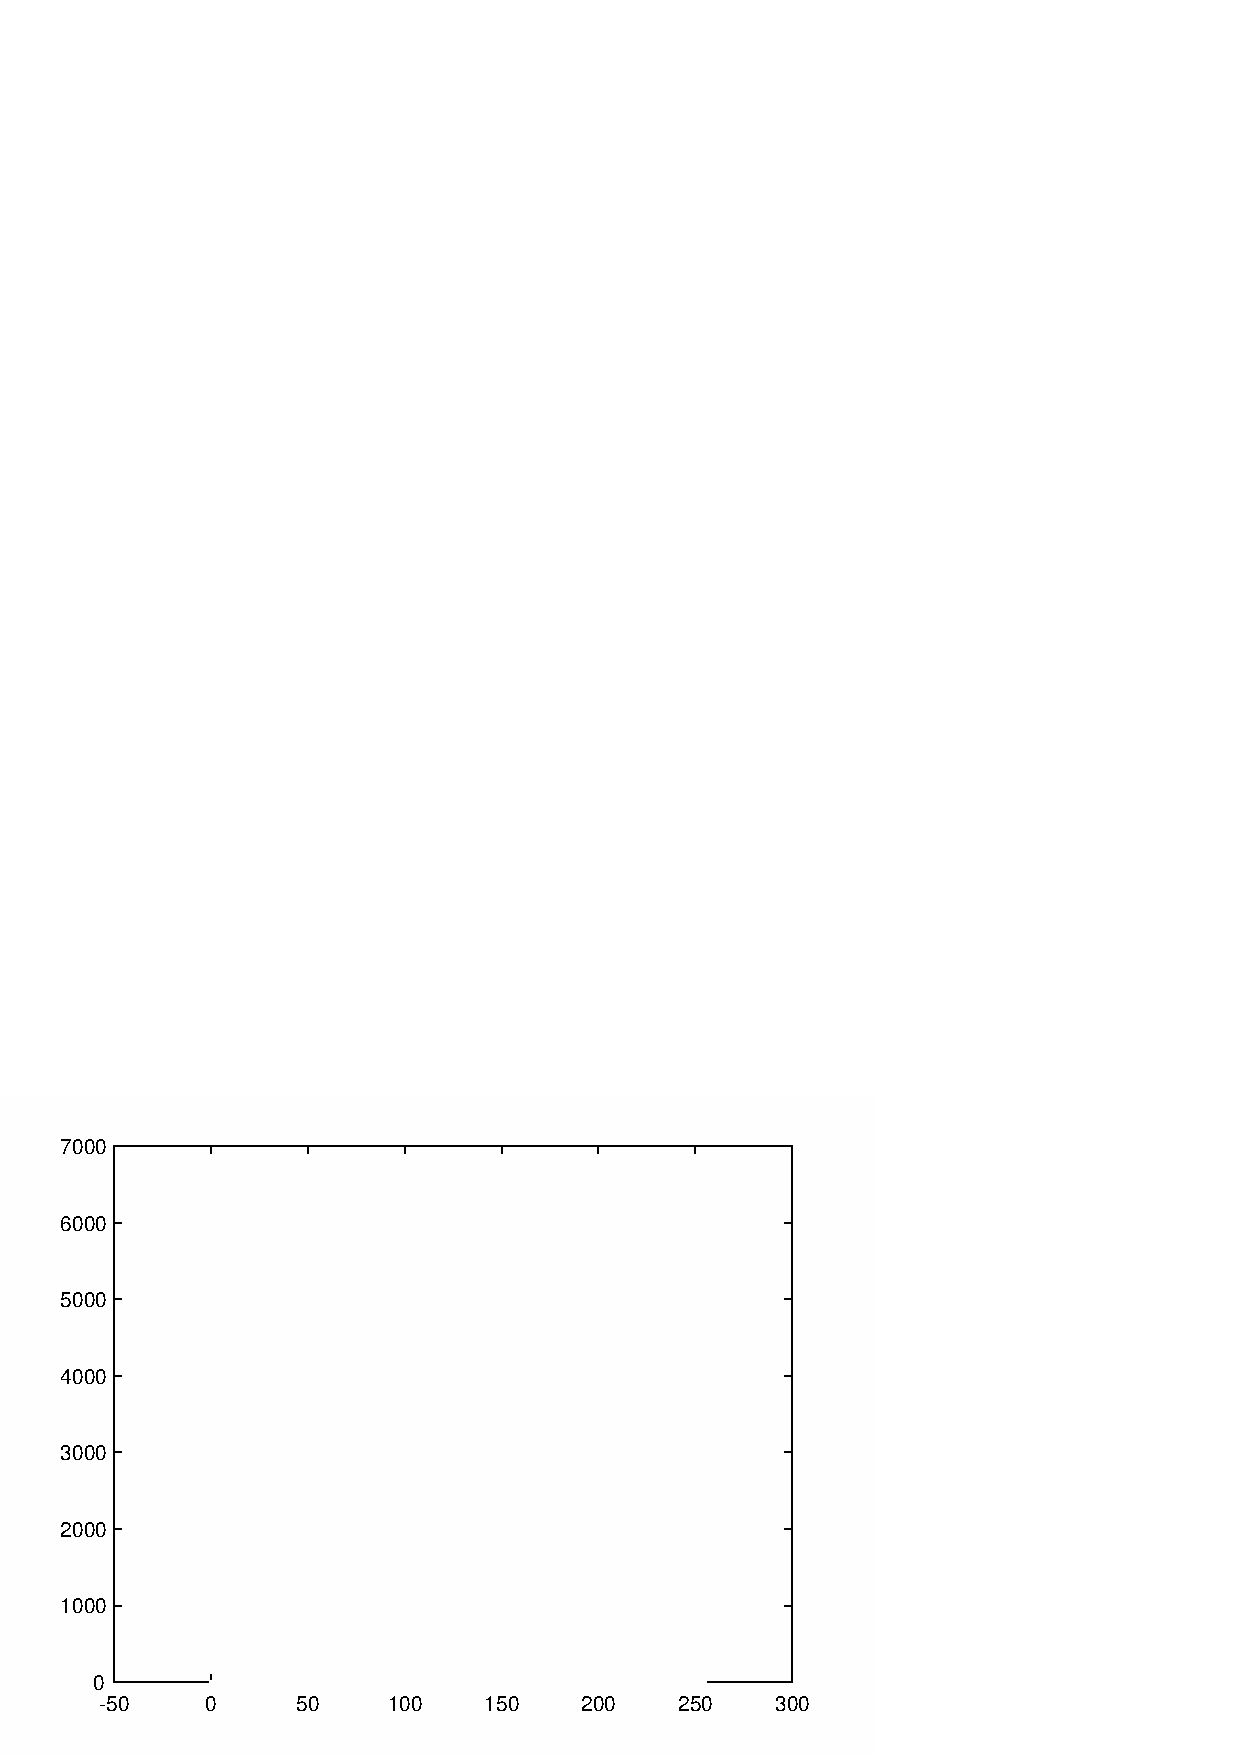
\includegraphics[width=\linewidth,  height = 5.5cm]{greenplane.jpg}
        \caption{}
        \label{green}
\end{subfigure}
\begin{subfigure}{.49\textwidth}
	\centering
        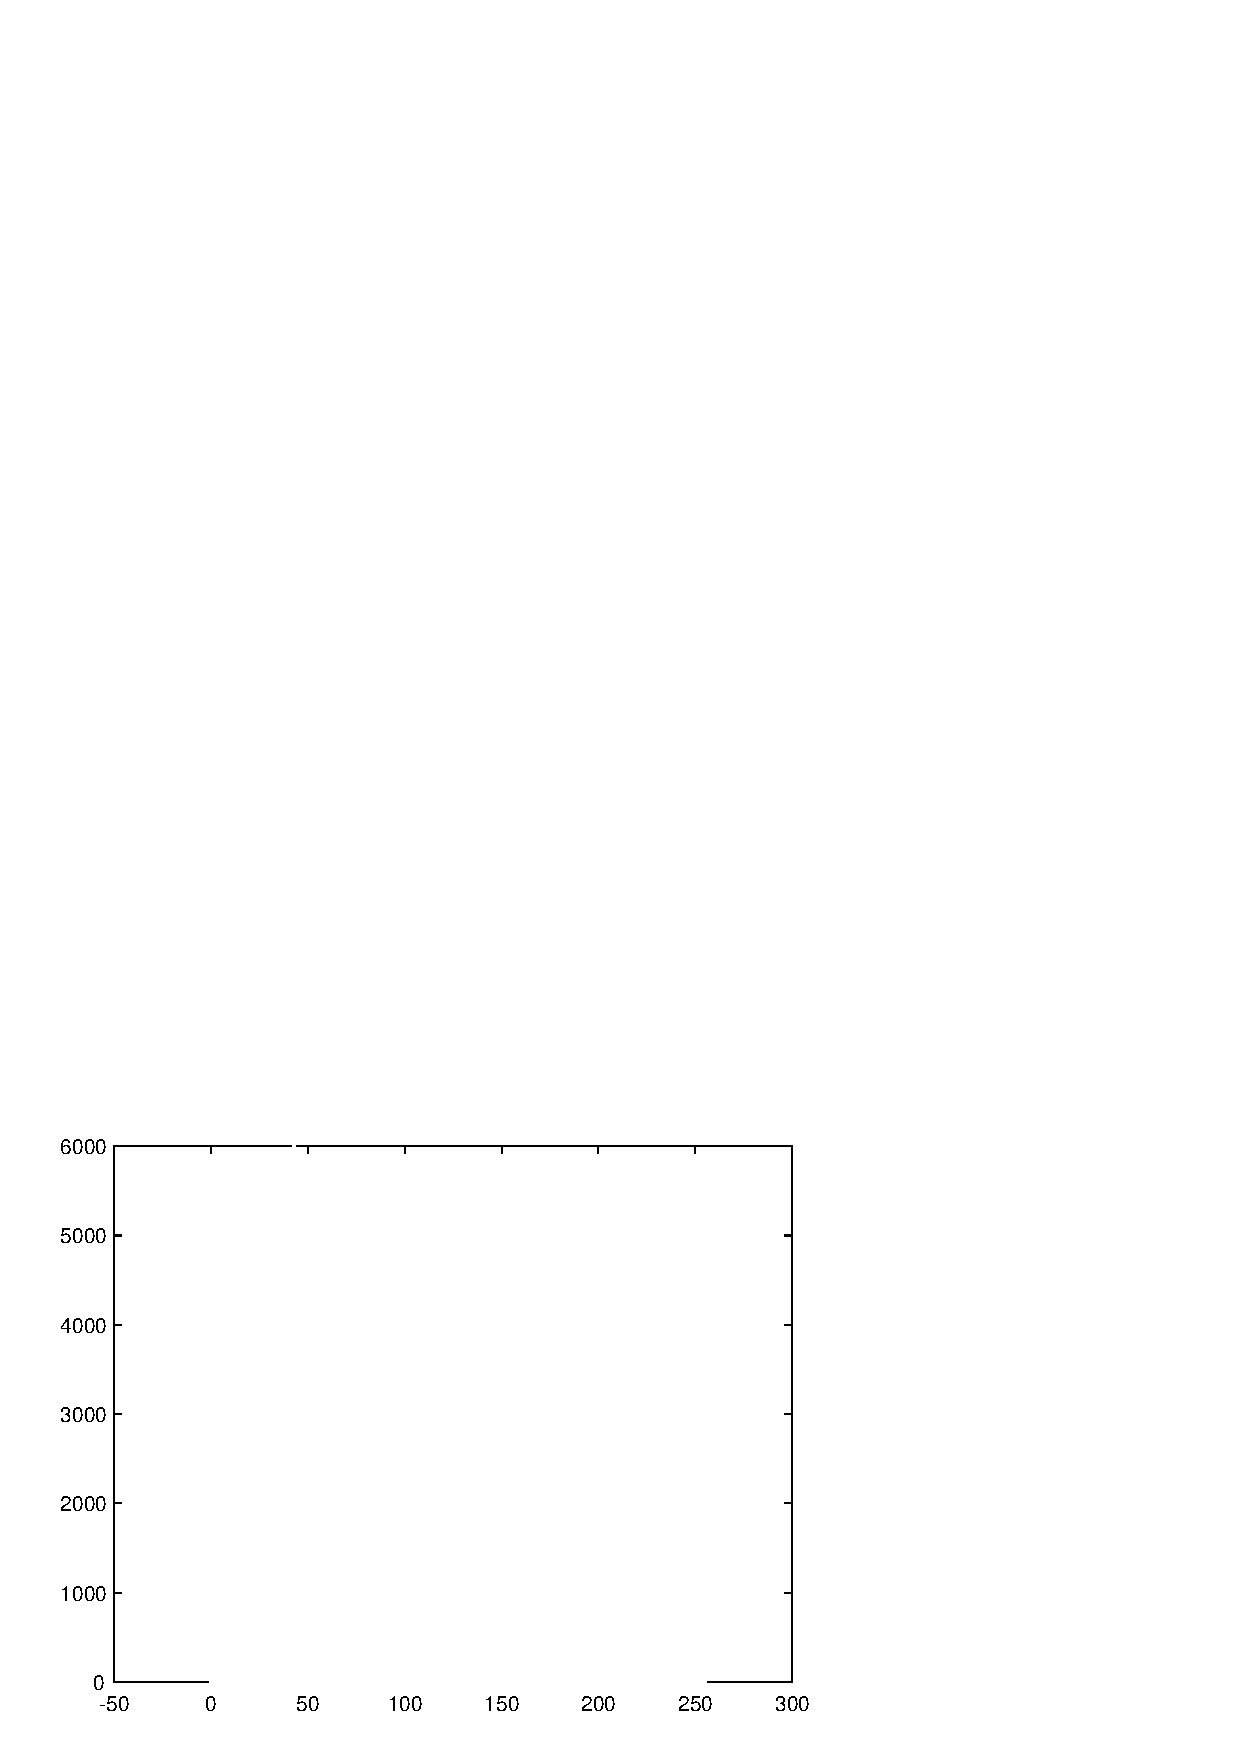
\includegraphics[width=\linewidth, height = 5.5cm]{blueplane.jpg}
        \caption{}
        \label{blue}
\end{subfigure}
\caption{(a): Red plane histogram, (b): Green plane histogram, (c): Blue plane histogram. The large peaks in each graph correspond to the pool table top.}
\label{pool}
\end{figure}

\newpage

%THRESHOLDING
\section{Thresholding}
To segment the green table in the image, the 3 colour planes were extracted from the complete image file. Three masks were then generated utilising the following thresholds: Red - min 0, max 120; Green - min 100, max 255; Blue - min 0, max 75. This created 3 logical matrices which were then combined and multiplied by each of the individual colour channels to filter out pixels of the image not included in the pool table top. However, this did not work perfectly, as can be seen in Figure \ref{newpool}. The body of the pool table was segmented well but the edges contain a lot of black pixels. This also occurs at the edges of the pool balls and the player's arm. This could be due to the change of colour between the pool table and these objects. Despite this, the overall shape of the pool table was preserved and the segmentation worked quite well. \\
\\
The segmentation was performed by applying a threshold to all 3 colour channels rather than just the green channel. This produces a better segmentation of the pool table. This is because if the only channel to be thresholded is green, then all of the pixels within the green the green thresholds that contain large amounts of blue and red, will appear on the image. This reduces the pool table quality and produces pixels of blue and red outside of the tabletop. Therefore, applying the threshold to all three channels will prevent these pixels passing the green threshold to be displayed, by blocking them with the red or blue channel thresholds / masks.

\begin{figure}[H]
\centering
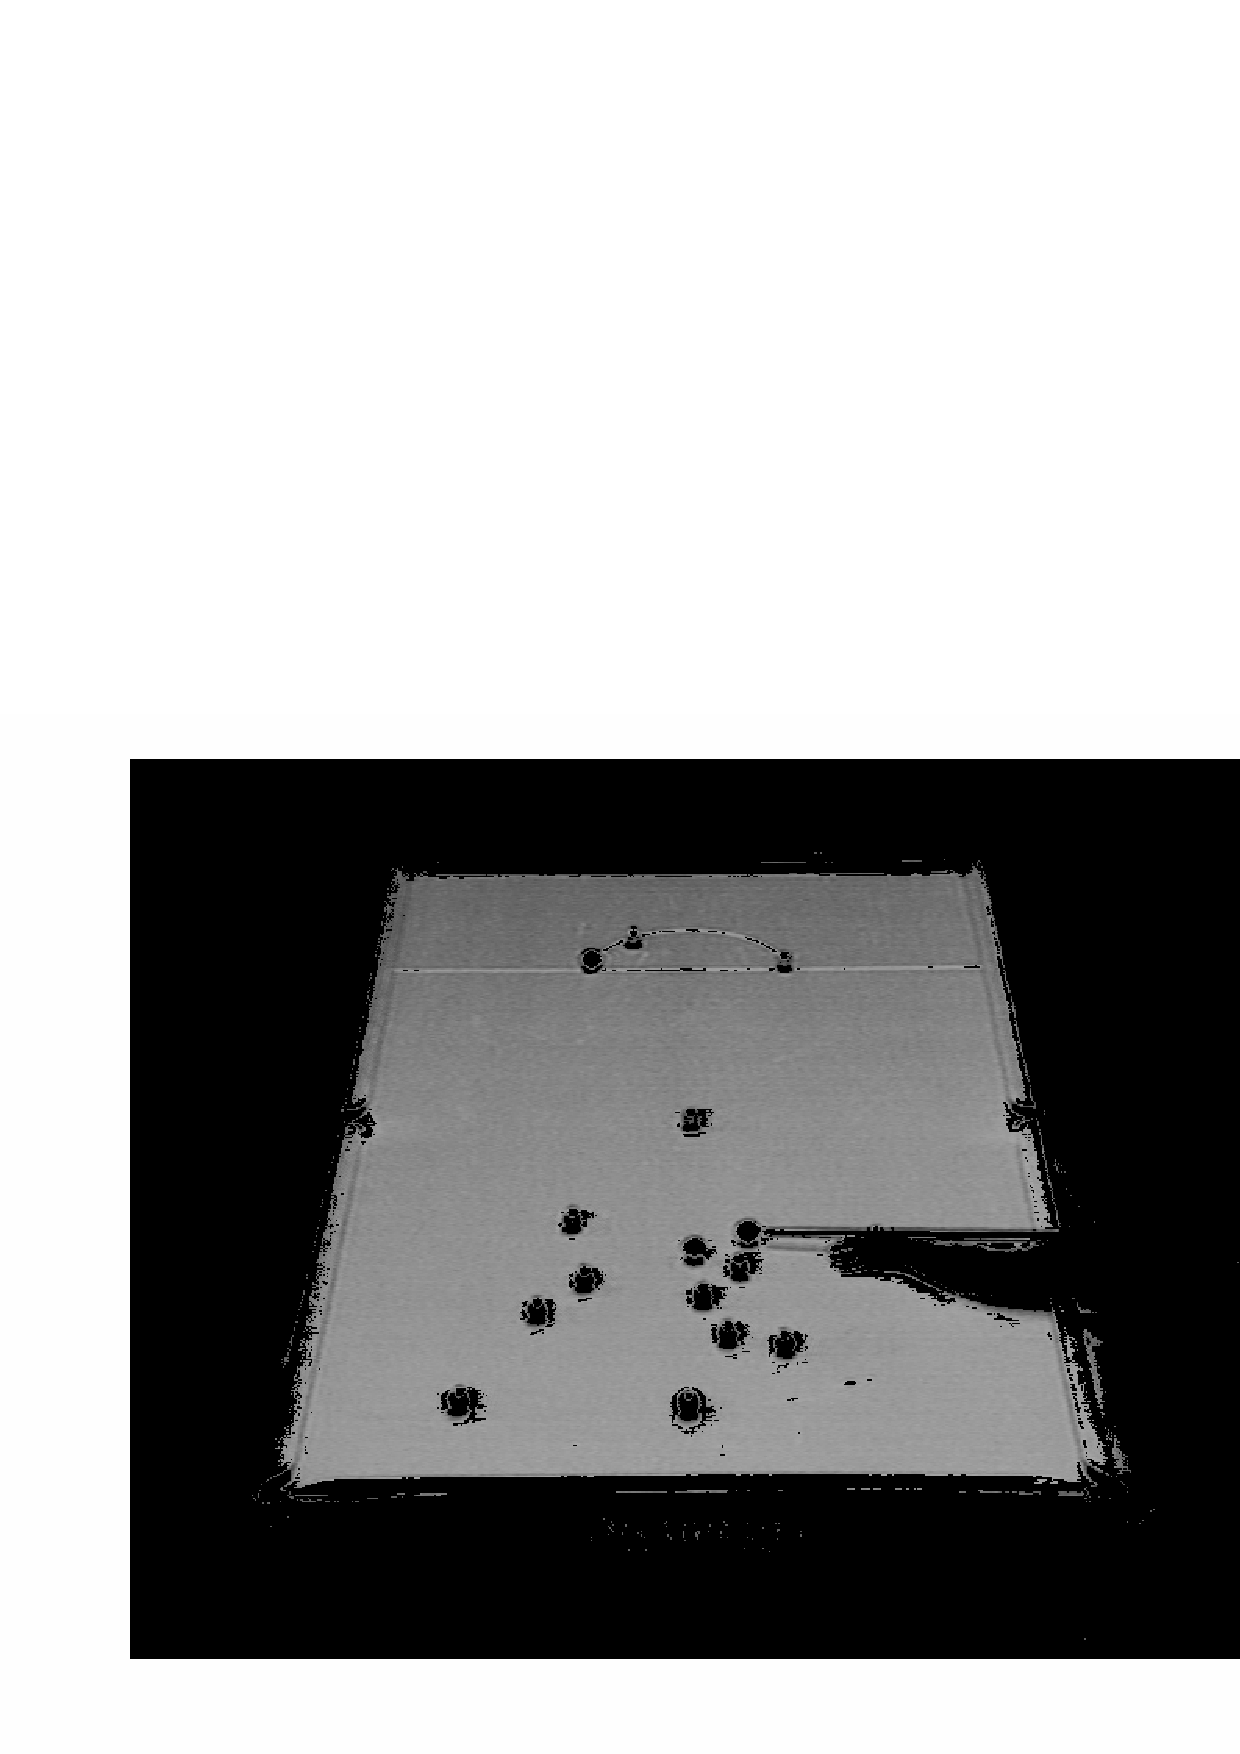
\includegraphics[width = \linewidth]{newpool.jpg}
\caption{Green tabletop of the pool table segmented in the image `pool.02.bmp'}
\label{newpool}
\end{figure}













\end{document}